
\chapter{METHODOLOGY}
{\baselineskip=2\baselineskip

In this chapter, the researchers detail the methodology employed to conduct the study, providing a comprehensive overview of the research design, data collection, and analytical procedures.

\section{Research Design}

\begin{figure}[H]
	\centering
	\caption{The Waterfall Model}
	\label{fig:waterfall}
	\includegraphics[width=1\textwidth]{figures/waterfall.png}
\end{figure}

In Figure 3.1, the system creation process is illustrated, utilizing a modified waterfall model. This systematic approach consists of several key stages, commencing with requirements gathering and followed by requirements analysis, hardware development, software development, system design, integration, and testing \& evaluation. This procedural framework acts as a guiding path for researchers to achieve the study's intended objectives.

\section{Planning}
\subsection{Research Setting}

\begin{figure}[H]
	\centering
	\caption{Map of Camiguin and Misamis Oriental}
	\label{fig:map}
	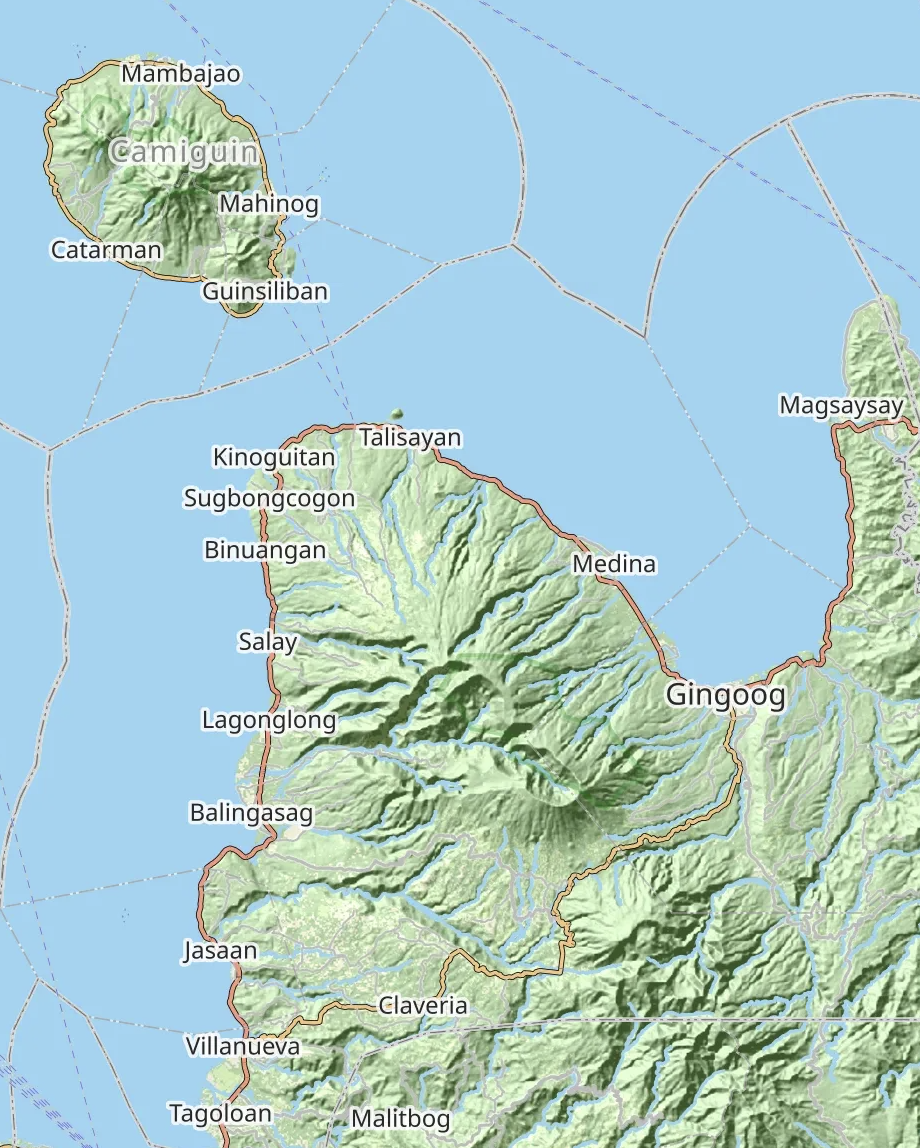
\includegraphics[width=0.7\textwidth]{figures/map.png}
\end{figure}

The research will be conducted in selected areas of Camiguin and Misamis Oriental, regions in the Philippines that are known for frequent and unscheduled power interruptions. These areas are served by CAMELCO (Camiguin Electric Cooperative) and MORESCO II (Misamis Oriental Electric Cooperative II), both of which experience regular power outages, particularly during peak hours. This issue disrupts daily activities, especially in community centers, educational institutions, and local businesses that rely on electricity for mobile devices, lighting, and small appliances.


\subsection{Data Collection}

The research team will gather data from both primary and secondary sources. For the primary data, first-hand interactions will be conducted with community residents, power supply providers, and solar energy experts. Community residents, as the primary users of the solar-powered rental station, will provide information on the demand for portable power sources, willingness to adopt a solar-powered system, and feedback on system usability and effectiveness in addressing power interruptions. Power supply providers, such as local electric cooperatives like CAMELCO and MORESCO 2, will provide data on the frequency of power interruptions, challenges in accessing reliable energy, and the overall energy demand in the community. Insights from solar energy experts will focus on technical aspects of solar power systems, including optimal photovoltaic panel configurations, energy storage solutions, and power inverter specifications.

Secondary sources will include academic papers, case studies, industry reports, and other literature related to solar energy, portable power stations, and renewable energy systems. These sources will provide a theoretical foundation and context for the study, ensuring that both practical relevance and technical feasibility are considered in developing the solar-powered rental station system.

\subsection{Data Gathering Procedure}

To obtain relevant qualitative data for the study, a series of in-depth interviews will be conducted with selected community residents using purposive sampling. The interviews will focus on understanding residents’ experiences with frequent power interruptions, the challenges they encounter during interruptions, and their perceptions of a solar-powered rental station as an alternative energy source. These discussions will also explore their reliance on backup power systems and their willingness to adopt renewable energy solutions. Participants will be purposively selected, particularly those who frequently experience power interruptions, depend on electricity for livelihood activities, and have expressed interest in solar technology. Combined with qualitative tools, this approach will ensure a comprehensive understanding of the community’s energy needs, user expectations, and potential areas for improving the design and implementation of the solar-powered rental station system.

\subsection{Data Finding Analysis}

The analysis of the collected data will lead to several important findings. The first will reveal that community residents frequently experience power interruptions that disrupt both household and livelihood activities. These interruptions will highlight common challenges related to the reliability, cost, and accessibility of backup power solutions. Residents will express concerns about their dependence on the unstable power grid and the lack of affordable alternatives during interruptions. The analysis will also uncover the community’s openness to adopting a solar-powered rental solution, recognizing its potential to provide a more sustainable and reliable energy source. Feedback from interviews and discussions will emphasize the need for practical improvements to the proposed system, such as flexible payment options (coin- or app-based), increased power capacity, and user-friendly accessibility. These insights will be vital in assessing the system’s feasibility and refining its design to ensure it effectively addresses the residents’ energy needs.

\section{Design}
\subsection{User Definition}

After the planning phase, the system’s users were identified. For this study, the Community Resident is defined as follows:

\textit{Community Resident - A person residing in a local community who is actively involved or has access to portable power sources during power interruptions or emergencies.}

\subsection{System Requirements}

\begin{longtable}{p{4cm} p{9cm}}
	\caption{System Requirements} \label{tab:SystemRequirements} \\
	\toprule
	\textbf{Category} & \textbf{System Requirement} \\
	\midrule
	\endfirsthead
	
	\toprule
	\textbf{Category} & \textbf{System Requirement} \\
	\midrule
	\endhead
	
	\bottomrule
	\endfoot
	
	Input Requirements & - The system shall collect user information during account registration through designated input fields in the mobile application. \\
	& - The system shall accept user login credentials such as username and password for authentication. \\
	& - The system shall accept rental requests, including power source selection, rental duration, and payment method (coin-based or app-based).\\
	& - The system shall receive telemetry data from each power source, including battery percentage, GPS location, and rental status through the GSM module. \\
	\midrule
	
	Process Requirements & - The system shall process rental transactions by verifying payment completion before authorizing power source access. \\
	& - The system shall generate and transmit an access token or unlock code to the power source upon successful rental approval. \\
	& - The system shall continuously monitor and record the battery level, location, and usage duration of active rentals. \\
	& - The system shall process the return of rented power sources by validating device ID, updating the database, and releasing the final transaction summary. \\
	\midrule
	
	Output Requirements & - The system shall display rental confirmation details such as power source ID, rental duration, and current charge level. \\
	& - The system shall provide real-time status updates on the mobile app, including remaining battery percentage, and device location. \\
	& - The system shall generate notifications for payment confirmation, overdue alerts, and successful returns. \\
	\midrule
	
	Control Requirements & - The system shall implement user authentication and authorization mechanisms to restrict access to registered users only. \\
	& - The system shall validate all rental and payment data to ensure that only completed and legitimate transactions are processed. \\
	\midrule
	
	Performance Requirements & - The system shall maintain fast response time during login, payment processing, and rental activation to ensure a smooth user experience. \\
	& - The system shall provide real-time monitoring and synchronization of power source data through reliable GSM and IoT communication.\\
	& -The system shall ensure continuous operation and high availability to prevent service interruptions during rentals. \\
\end{longtable} 

\subsection{System Design and Architecture}

\begin{figure}[H]
	\centering
	\caption{System Architecture}
	\label{fig:architecture}
	\includegraphics[width=1\textwidth]{figures/architecture.png}
\end{figure}

Figure 3.3 illustrates the architecture of the KuRyenta system, a solar-powered, coin-operated, GPS-enabled portable power source. The diagram shows how solar energy is captured by the photovoltaic panels and stored in a \ce{LiFePO4} battery through the solar charge controller. The stored energy is then converted into usable AC power by the power inverter, which is accessible to the user via a coin-operated access system.

The ESP32 microcontroller manages the system's operations, integrating key components such as the GPS module for location tracking and the GSM module for communication with the admin. A coin slot and solenoid lock control the unlocking of the portable power sources, ensuring that users can access the power only after payment is made. The user can interact with the system through a mobile app that displays the battery's charge level and other important information. In essence, the KuRyenta system is designed to provide a sustainable and secure solution for portable power, incorporating solar energy, and coin-based access for a user-friendly and efficient experience.


\subsection{System  Flowchart}
\begin{figure}[H]
	\centering
	\caption{System Flowchart}
	\label{fig:flowchart}
	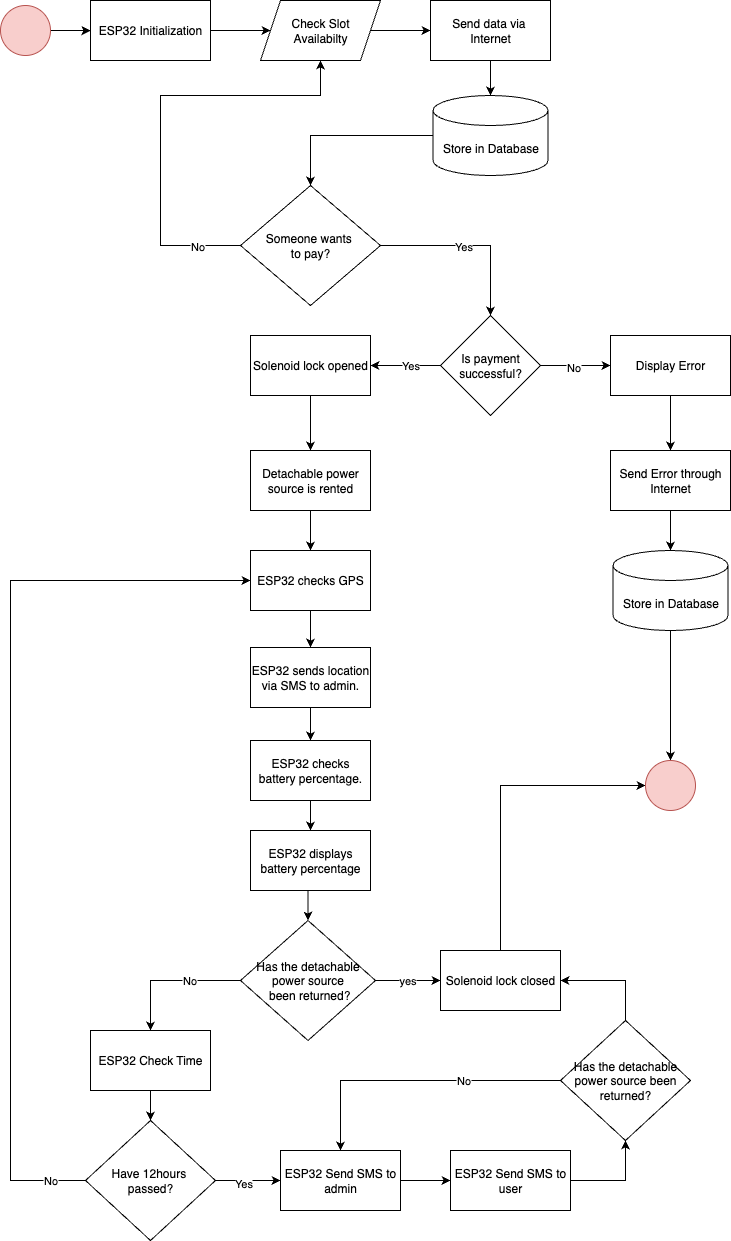
\includegraphics[width=0.7\textwidth]{figures/flowchart.png}
\end{figure}

Figure 3.4 illustrates the overall process of the proposed Solar-Powered Rental Station with Detachable Power Sources. The process begins with the initialization of the ESP32, which activates system components and prepares communication protocols. The system first checks slot availability to determine if a detachable power source is ready for use. Data from this process is transmitted through the internet and stored in a central database for monitoring purposes.

When a user intends to rent a power source, the system verifies if payment is successful. If confirmed, the solenoid lock opens, allowing the detachable power source to be accessed by the user. Once rented, the ESP32 continuously monitors the power source, including its GPS location and battery percentage, and sends the information to the administrator via SMS. This ensures proper tracking and security of the rented device.

The system also monitors whether the detachable power source is returned. If it remains unreturned after 12 hours, the ESP32 automatically sends reminder SMS notifications to both the user and the administrator. Upon return, the solenoid lock closes, securing the power source back in place. All key actions, including errors and system activities, are logged in the database for reference and analysis.


\subsection{Solar Energy Harvesting}

\begin{figure}[H]
	\centering
	\caption{Conversion of Sunlight into Electrical Energy using PV Panels and a Charge Controller}
	\label{fig:solar harvesting}
	\includegraphics[width=1\textwidth]{figures/harvesting.png}
\end{figure}

The Figure 3.5 illustrates the process of harvesting solar energy using photovoltaic (PV) panels. Solar energy is captured by the PV panels, which then convert sunlight into electrical energy. The energy is stored in a \ce{LiFePO4} battery through a solar charge controller, ensuring proper charging and voltage regulation. This energy is stored for later use, contributing to the overall sustainability and efficiency of the system, enabling it to power devices even during periods of limited sunlight.

\subsection{Energy Conversion DC to AC}

\begin{figure}[H]
	\centering
	\caption{Battery DC power converted to AC output via Inverter.}
	\label{fig:energy conversion}
	\includegraphics[width=1\textwidth]{figures/conversion.png}
\end{figure}

Figure 3.6 shows the process of converting direct current (DC) into alternating current (AC). The stored energy in the \ce{LiFePO4} battery is passed through a power inverter, and the inverter transforms the DC from the battery into AC power, which can be used to power household appliances such as fans and other AC-powered devices. This conversion is essential for making the system compatible with common electrical appliances that require AC power for operation.

\subsection{Power Monitoring}

\begin{figure}[H]
	\centering
	\caption{ESP32 measures battery voltage and displays data on LCD}
	\label{fig:power monitoring}
	\includegraphics[width=1\textwidth]{figures/monitoring.png}
\end{figure}

The Figure 3.7 illustrates the power monitoring system used to keep track of the energy stored and consumed by the system. The \ce{LiFePO4} battery is connected to an ESP32 microcontroller, which continuously monitors the battery’s voltage and health, and the data collected is displayed on an LCD screen which allows users to view the battery's current status in real time. This monitoring is vital for ensuring the system's efficiency and preventing over-discharge, ensuring long-term sustainability.


\subsection{GPS Tracking}

\begin{figure}[H]
	\centering
	\caption{ESP32 receives real-time location data from GPS satellites using GSM Module}
	\label{fig:gps tracking}
	\includegraphics[width=1\textwidth]{figures/tracking.png}
\end{figure}

Figure 3.8 shows the GPS tracking system used to monitor the location of the detachable power source. A GPS module, connected to the ESP32 microcontroller, receives signals from satellites to determine the geographical location of the system. This real-time location data is essential for tracking and managing the rental and use of the power sources, ensuring they are accessible to users and protected from theft or misuse. The GPS data is then sent to the system for further processing and user access.


\section{Develop}

\subsection{Context Level Diagram}

\begin{figure}[H]
	\centering
	\caption{Context Level Diagram}
	\label{fig:context level diagram}
	\includegraphics[width=\textwidth]{figures/context.png}
\end{figure}

This Figure 3.9 illustrates the Context Level Diagram of the system. The Mobile App serves as the primary interface through which Community Residents interact with the Solar-Powered Rental Station. The Community Resident starts by providing their registration information via the Mobile App, which sends this data to the system. Once registered, the system sends back a registration confirmation and the Mobile App allows users to proceed with rental/payment requests. The Mobile App then facilitates payment transactions where the Community Resident can complete the payment either through a coin-based mechanism or an app-based method. Once the payment transaction is successfully completed, the Mobile App receives a payment confirmation from the System, ensuring the rental is validated. The Community Resident can then use the Mobile App to check the system status, such as battery levels, power source availability, or the remaining rental time. After use, the Community Resident sends a return request via the Mobile App, which then communicates with the System to confirm the power source return. The System logs the return and ensures the process is validated, signaling the completion of the rental session. Additionally, the Mobile App allows the Community Resident to submit feedback on their experience with the service.

On the other side, the System (the Solar-Powered Rental Station) manages the backend of the rental process. It verifies rental requests from Community Residents and authorizes them to rent a power source. It also handles payment processing, ensuring that the payment is verified before the rental is completed. Once payment is confirmed, the System updates the Mobile App with the confirmation. The System also monitors the rented power source, providing live monitoring information, such as the power source’s battery level and available runtime. If the Community Resident fails to return the power source on time or if the power source is running low on battery, the System sends low battery or overdue alerts to both the Mobile App and the Community Resident, prompting them to take action. 

\subsection{Data Flow Diagram}
\begin{figure}[H]
	\centering
	\caption{Data Flow Representation of the Solar-Powered Rental Station System}
	\label{fig:data flow}
	\includegraphics[width=1\textwidth]{figures/dataflow.png}
\end{figure}
	
The Figure 3.10 shows the complete process flow of the solar-powered rental station system, illustrating how community residents interact with the mobile application and system database. It begins with the login process, where residents input their login details, which are verified by the system. Once authenticated, the system provides feedback confirming successful login. After logging in, the user proceeds to make a rental request by selecting a power source and specifying the rental duration. The system responds with rental confirmation and product details. The user then moves to the payment process, where payment details are submitted through the app. The system validates the payment, sends a confirmation, and generates an access token that authorizes the user to unlock and use the detachable power source.

Once access is granted, the rental authorization and monitoring phase begins. The system continuously provides updates on the power source’s status, such as battery level and remaining usage time, ensuring that the user can track energy consumption. When the rental period ends, the user then sends a return request, and the system verifies and confirms the return while updating the rental status. After returning the power source, the user proceeds to the feedback process, submitting performance feedback through the app. The system stores the feedback and confirms successful submission. After that, the system records the final rental summary and sends any overdue alerts if the power source is not returned on time. Overall, the diagram presents a clear and structured view of how the user’s actions and system responses are linked throughout the entire rental transaction cycle, which is from login to feedback completion.

\subsection{Use Case Diagram}
 \begin{figure}[H]
 	\centering
 	\caption{Use Case Diagram}
 	\label{fig:use case}
 	\includegraphics[width=1\textwidth]{figures/usecase.png}
 \end{figure}
 
Figure 3.11 illustrates how different users and administrators interact with the system. It highlights the actions users can take and the roles of administrators. The Unregistered User is someone who has not yet signed up for the system. They can create an account by providing their details, which are then verified by the system. If the details are correct, an activation code is generated for the user to complete the registration. After signing up, the user can log in to the system, but if there’s an issue with the login, an error is displayed.
 
 Once the Unregistered User becomes a Registered User after logging in successfully, they can perform more actions within the system. The user can rent a power source by checking its availability, paying for it, and activating the slot where the power source is stored. If there’s a problem with communication during the rental process, the system handles this as an extended action. After using the power source, the user can return it, and the system confirms the return. If there’s any delay in returning the power source, the system will manage this as well. Registered users also have the ability to view their account details and rental history, and they can report any issues or provide feedback through the system. The Admin plays a key role in overseeing the system. They can manage users, including adding or removing them from the system. The admin is also responsible for performing system updates and maintenance, ensuring the smooth operation of the system. Additionally, the admin can view various reports that provide insights into system performance and user activities.
 
 The relationships in the diagram are shown through Include and Extend. Include means that one action is always linked to another. For example, signing up always includes verifying the user's details, and renting a power source includes checking availability and processing payment. Extend means that certain actions may trigger additional steps under specific conditions. For instance, if a payment fails, it will trigger the "Payment Error" action, or if the power source return is delayed, it will trigger the "Return Delay" action. In summary, this use case diagram provides an overview of how users and administrators interact with the system, covering key actions like renting and returning power sources, managing user accounts, and maintaining the system.
 
 \subsection{Activity Diagram}
  \begin{figure}[H]
 	\centering
 	\caption{Activity Diagram of the Community Resident}
 	\label{fig:activity}
 	\includegraphics[width=0.7\textwidth]{figures/activity.png}
 \end{figure}
 
Figure 3.12 shows the step-by-step activity flow of the system from user login to unlocking the portable power source. The process begins with checking account availability. If the user already has an account, they proceed to the login step; otherwise, they must sign up first. After logging in, the system checks if the account is valid. If the account is invalid, the process returns to the login step. If valid, the system verifies the account and displays the dashboard. Next, the system checks if a power source slot is available. If no slot is available, the user remains on the dashboard until one becomes free. If a slot is available, the process continues to the payment step. The system then verifies the payment amount. If the amount entered is not exact, the process returns to the payment step. If the payment is correct, the portable power source is successfully unlocked, completing the process.
 
 Overall, the diagram clearly shows how the user interacts with the system , which starts from account access, validation, and payment, up to unlocking the rented portable power source.

   
  \subsection{3D Design}
  
    \begin{figure}[H]
  	\centering
  	\caption{Three Dimensional Representation of the System}
  	\label{fig:3d}
  	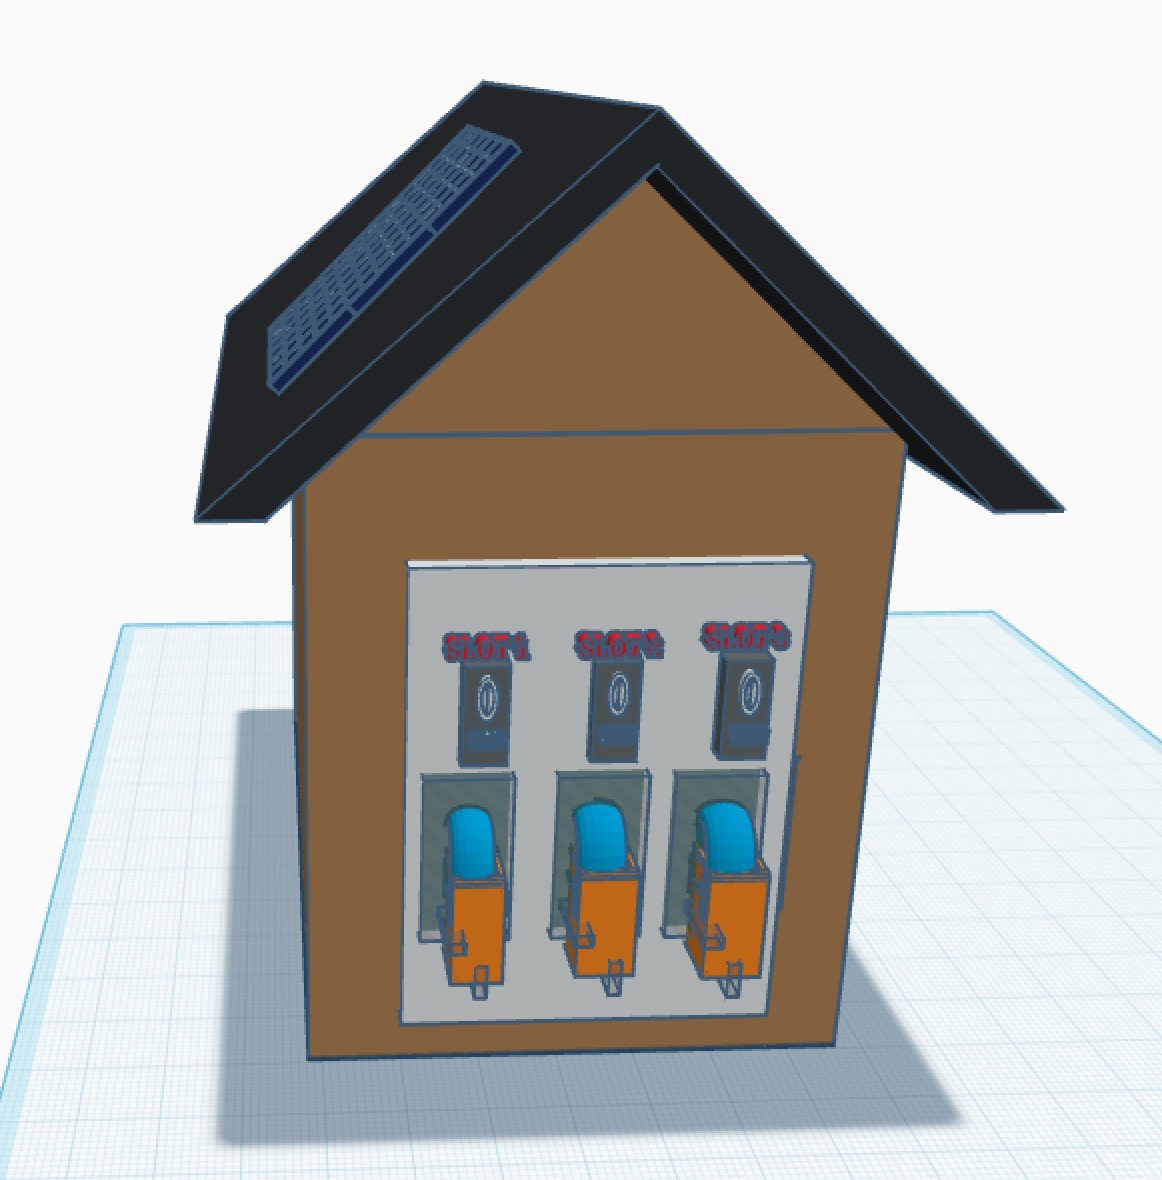
\includegraphics[width=0.8\textwidth]{figures/3D.png}
  \end{figure}
  
Figure 3.13 shows the 3D design of the system. It is a stationary power station powered by solar energy and contains three detachable power sources, each secured with a coin slot and solenoid lock.
  
  \subsection{Mobile App}
  
     \begin{figure}[H]
  	\centering
  	\caption{Welcome Page}
  	\label{fig:welcome}
  	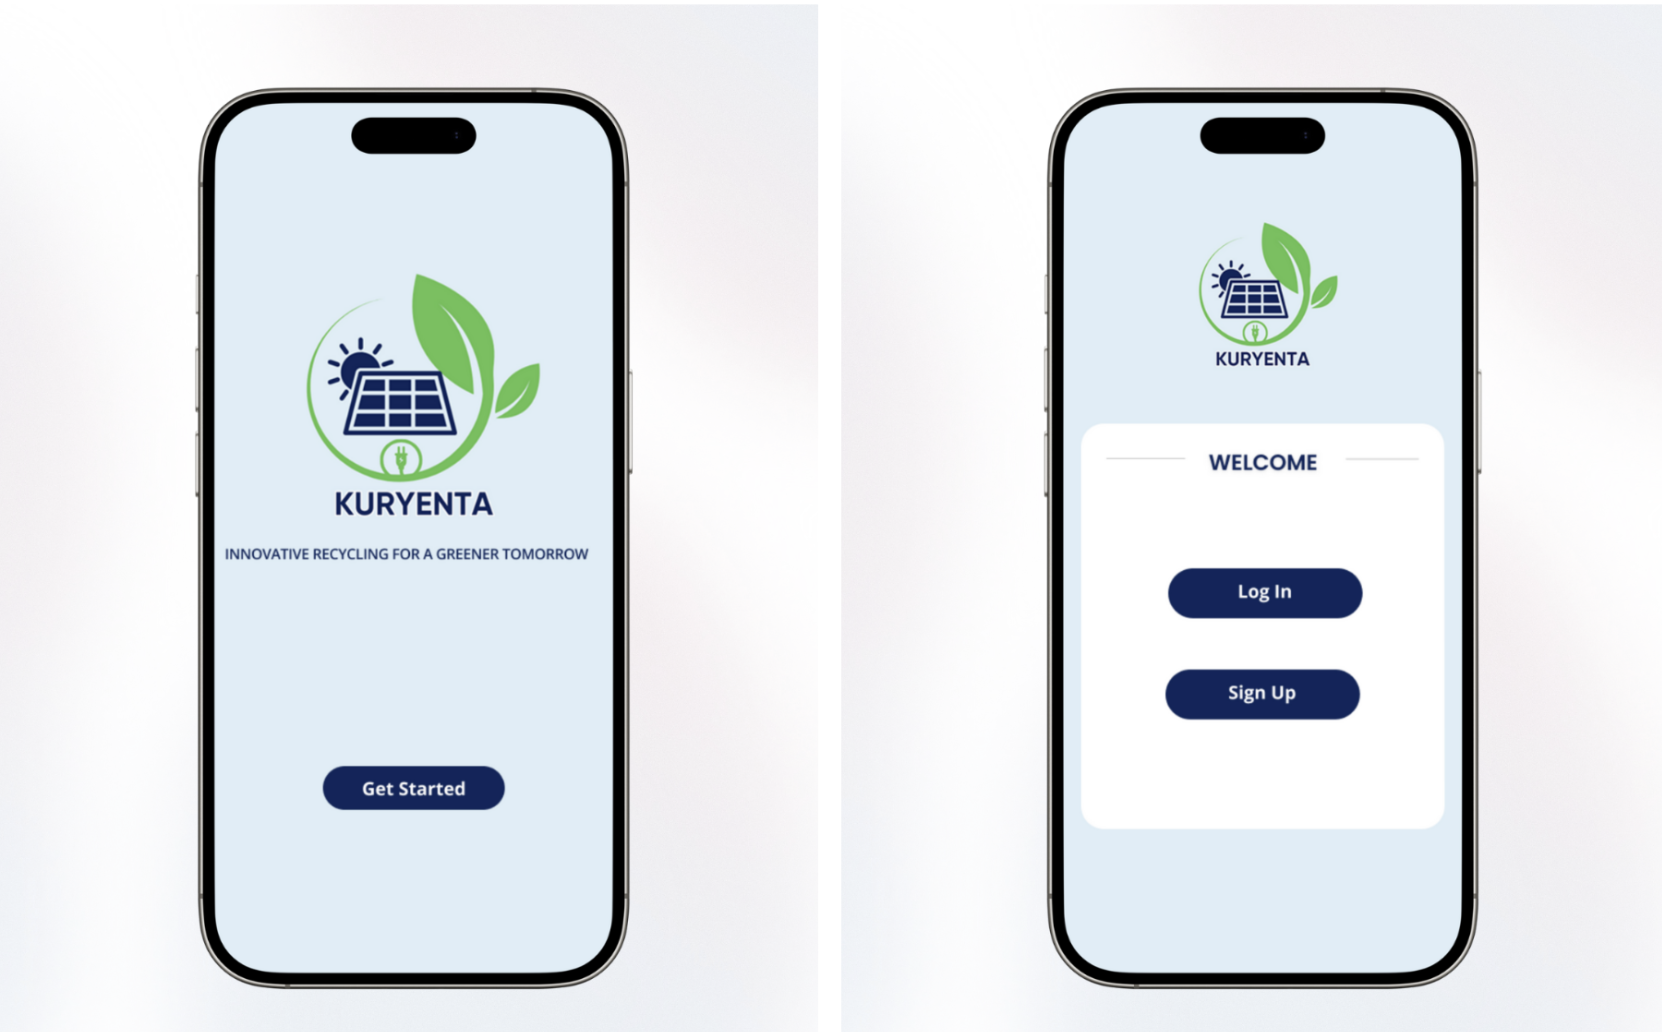
\includegraphics[width=1\textwidth]{figures/welcome.png}
  \end{figure}
  
  The welcome interface presents the system logo and entry actions. The left panel shows a splash screen with a “Get Started” control; the right panel shows a gateway card offering Log In and Sign Up. This screen functions as the access point to the authentication flow.
  
   \begin{figure}[H]
  	\centering
  	\caption{Sign n Screen}
  	\label{fig:signin}
  	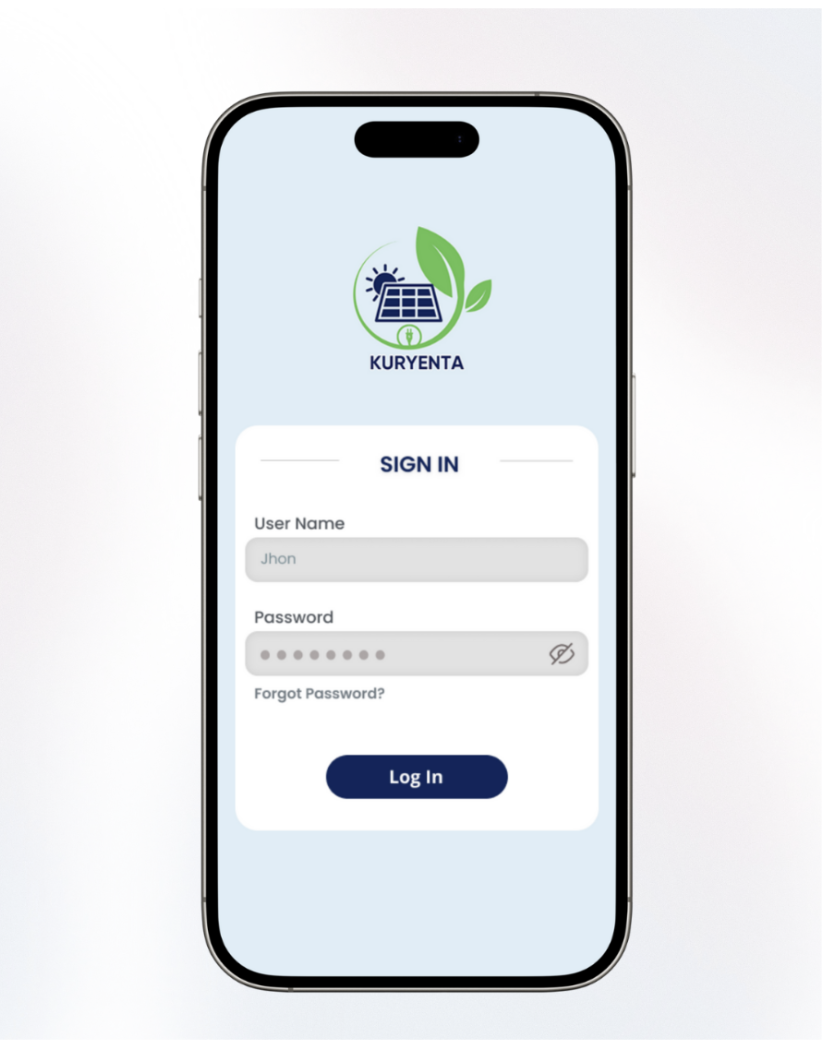
\includegraphics[width=0.7\textwidth]{figures/signin.png}
  \end{figure}
  
  The sign-in interface collects the username and password with options to reveal the password and recover forgotten credentials. A primary Log In control initiates authentication for registered users. The design supports secure access to user functions.
  
   \begin{figure}[H]
  	\centering
  	\caption{Sign Up Screen}
  	\label{fig:signup}
  	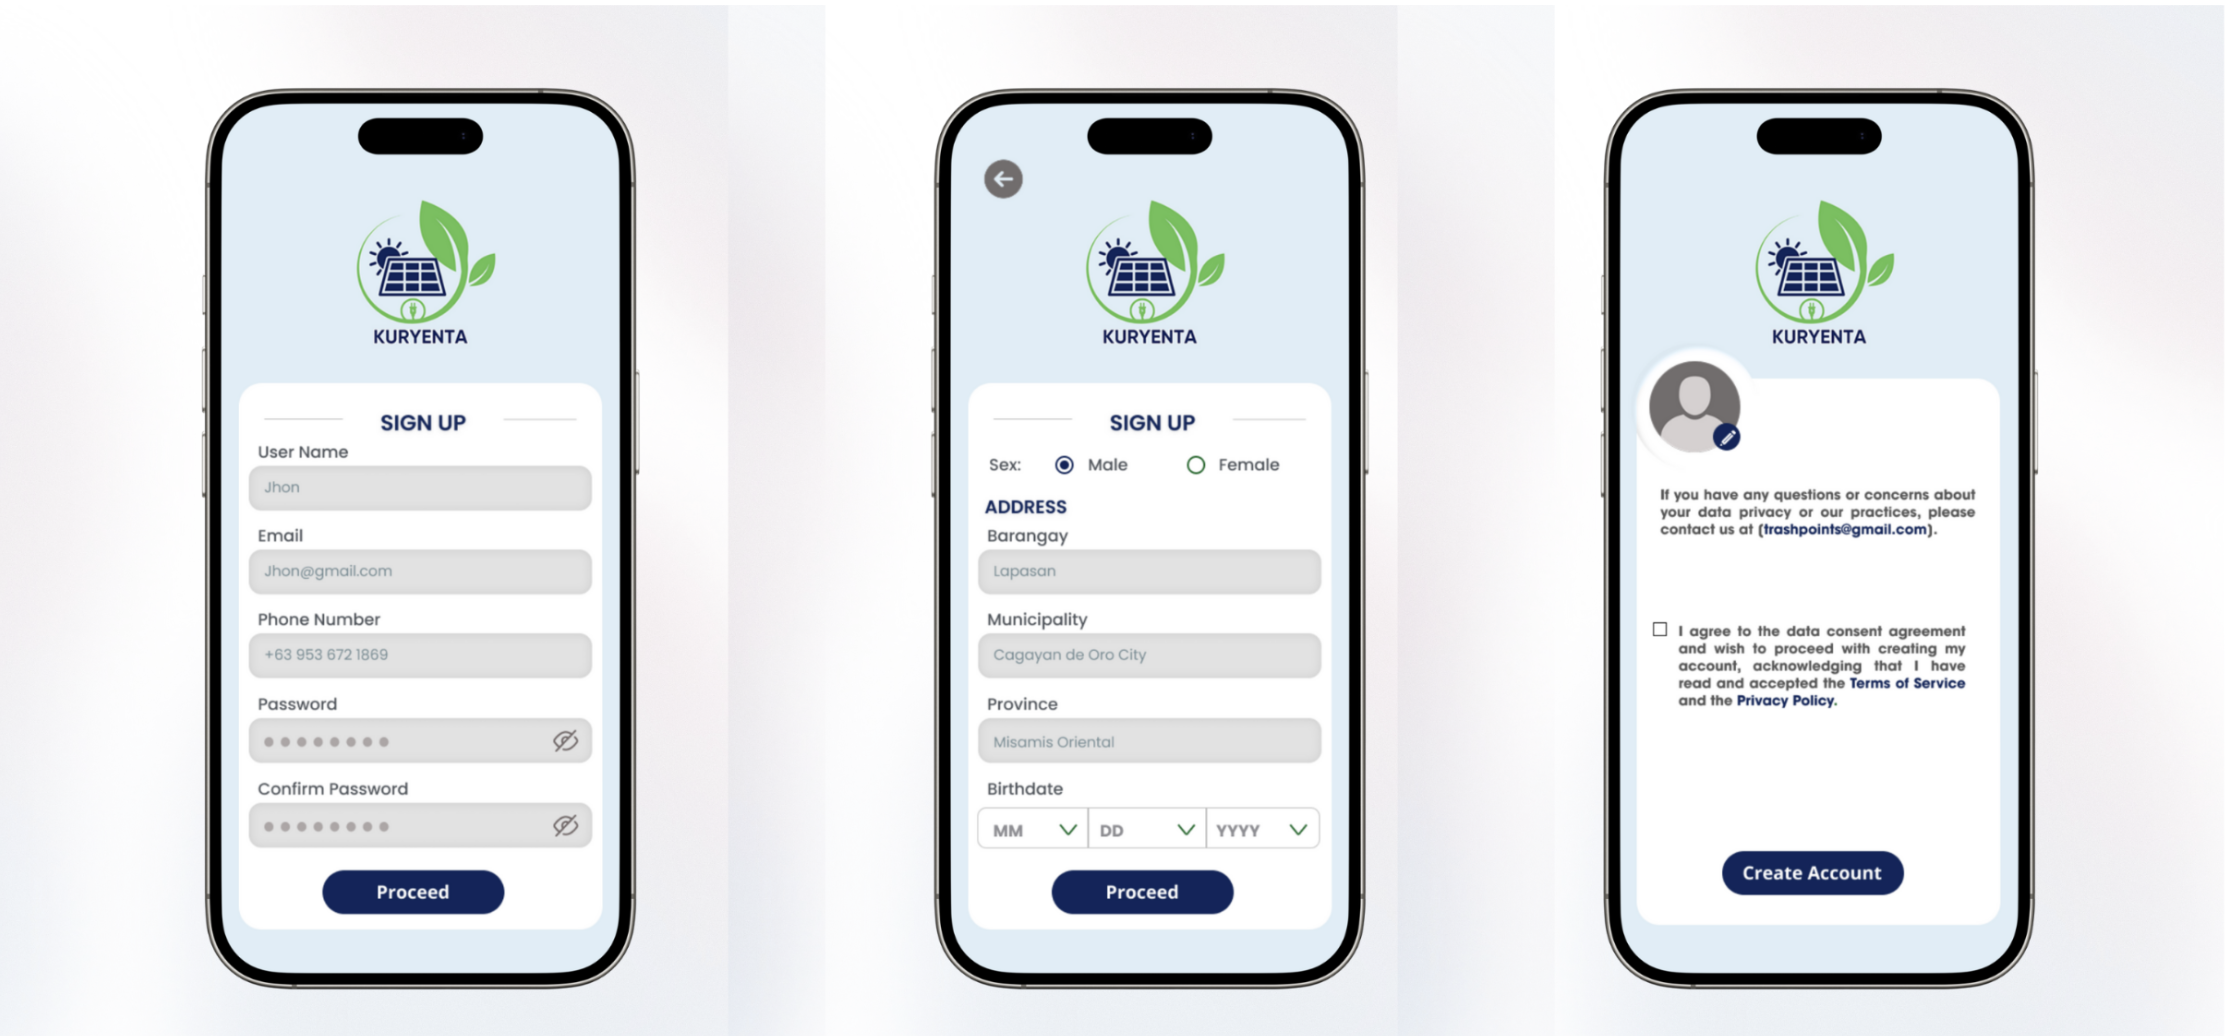
\includegraphics[width=1\textwidth]{figures/signup.png}
  \end{figure}
  
  Registration is implemented as a three-step process. Step 1 captures account credentials (username, email, phone number, password, and confirmation). Step 2 records profile and address data (sex, barangay, municipality, province, and birthdate). Step 3 presents a data-privacy notice and obtains consent to the Terms of Service and Privacy Policy before account creation.
  
    \begin{figure}[H]
  	\centering
  	\caption{User Home Screen}
  	\label{fig:user home}
  	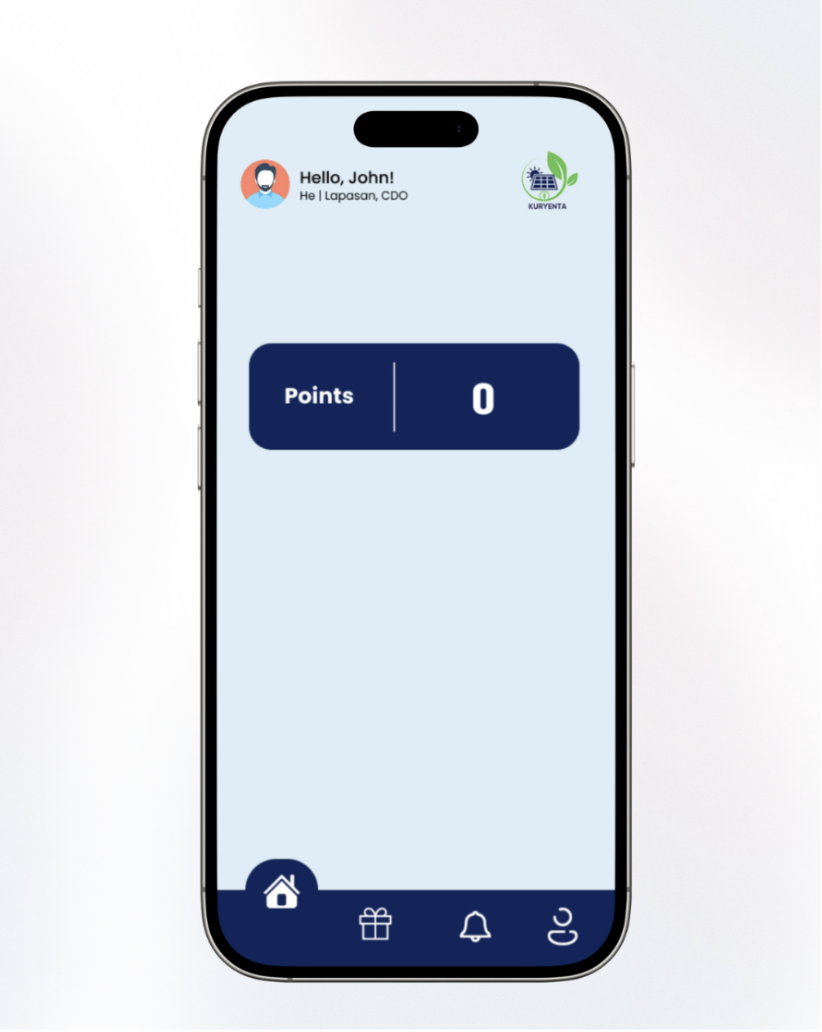
\includegraphics[width=0.7\textwidth]{figures/home.png}
  \end{figure}
  
  The user dashboard displays a greeting header with location metadata and a card showing the current points balance. A bottom navigation bar provides access to core modules (home, rewards, notifications, and account/tools). This screen serves as the primary hub for user activities.
  
    \begin{figure}[H]
  	\centering
  	\caption{Renting Screen}
  	\label{fig:renting}
  	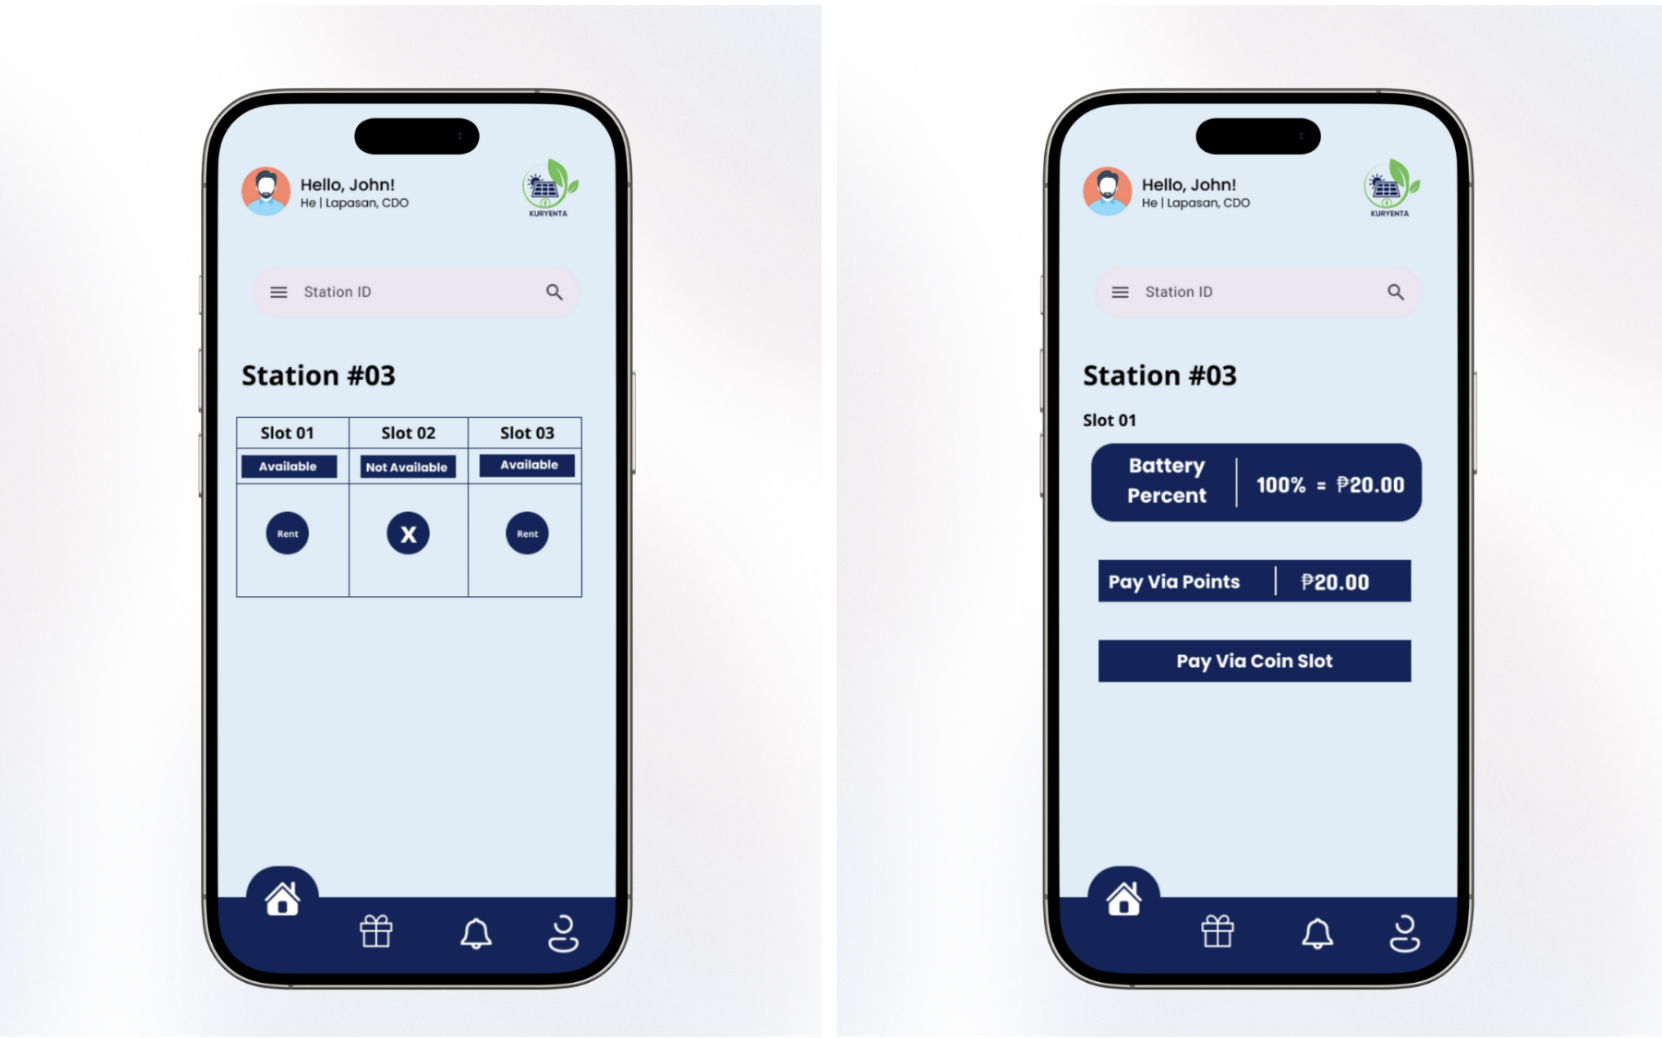
\includegraphics[width=1\textwidth]{figures/renting.png}
  \end{figure}
  
  The renting module allows search by Station ID and shows slot availability per station. Users select a slot and view its battery percentage with the corresponding price. Payment options include Pay via Points and Pay via Coin Slot, enabling transaction initiation.
  
  \begin{figure}[H]
  	\centering
  	\caption{Admin Home  Screen}
  	\label{fig:admin}
  	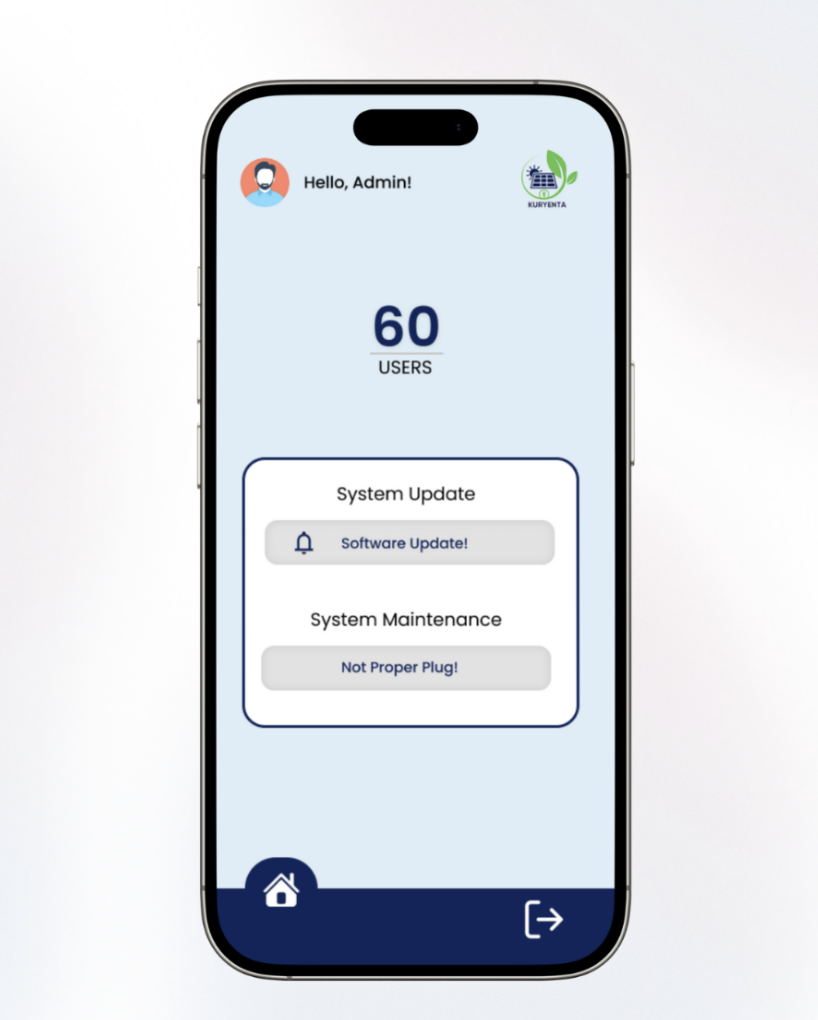
\includegraphics[width=0.3\textwidth]{figures/admin.png}
  \end{figure}
  
  The administrative dashboard reports the total number of users and provides status cards for system updates and system maintenance alerts. A bottom navigation enables movement to other administrative functions. This screen supports monitoring and operational control.
  
      \begin{figure}[H]
      	\centering
      	\caption{Admin Manage Users Screen}
      	\label{fig:admin2}
      	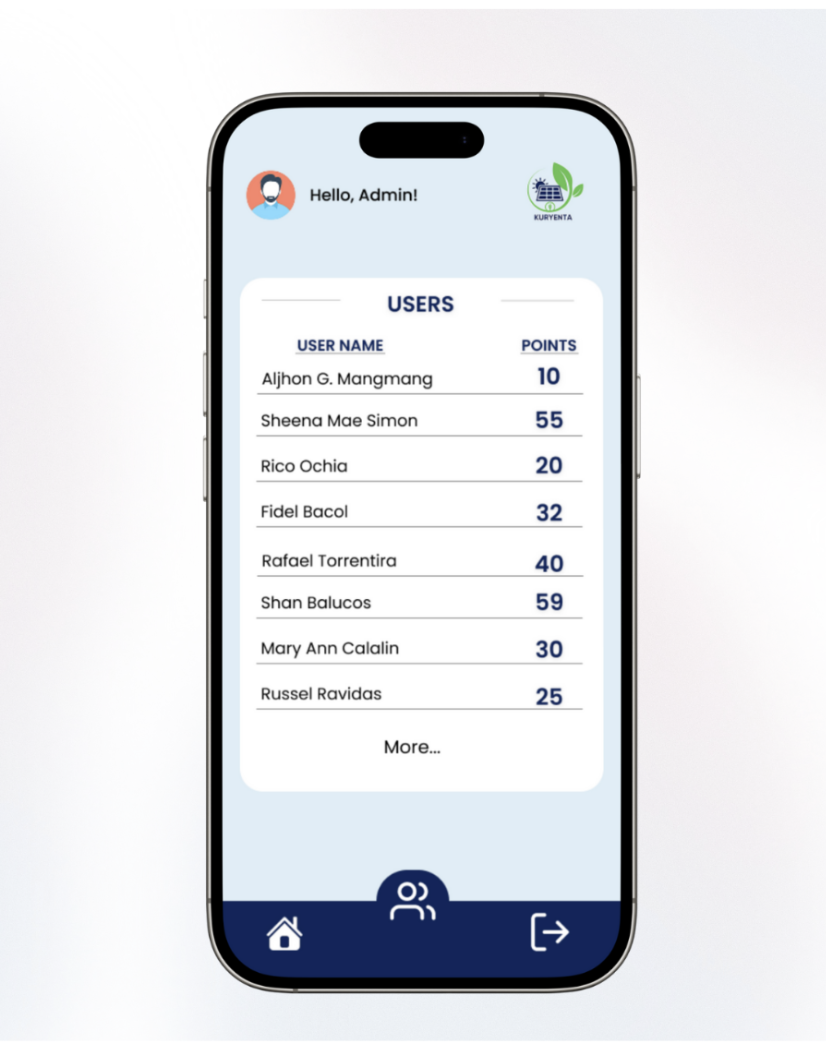
\includegraphics[width=0.3\textwidth]{figures/admin2.png}
      \end{figure}
      
      The user-management view lists registered users with their points balances. The list supports further exploration through a “More…” action. This screen enables oversight of accounts for incentive tracking and administration.
      
      
 \subsection{Materials and Cost}
     
     \begin{longtable}{p{6cm} p{4cm}}
     	\caption{Hardware Components and Cost} \label{tab:MaterialsAndCost} \\
     	\toprule
     	\textbf{Component} & \textbf{Price} \\ 
     	\midrule
     	\endfirsthead
     	
     	\toprule
     	\textbf{Component} & \textbf{Price} \\ 
     	\midrule
     	\endhead
     	
     	\bottomrule
     	\endfoot
     	
     	Battery x 2 & \textpeso 12,000.00 \\ 
     	Solar Charge Controller & \textpeso 1,000.00 \\ 
     	Solar Panel & \textpeso 2,500.00 \\
     	Pure Sine Wave Inverter x 2 & \textpeso 6,000.00 \\
     	Lithium Battery  Charger & \textpeso 500.00 \\
     	Low Voltage Disconnect module & \textpeso 100.00 \\
   	    Coin Slot Facade & \textpeso 150.00 \\
     	ESP32 x 2 & \textpeso 400.00 \\
     	DC breaker x 3 (Cable, Mounts) & \textpeso 100.00 \\
     	Relay Module 12/ 240v   x 2 & \textpeso 240.00 \\ 
     	Liquid Crystal Display (LCD) x 2 & \textpeso 400.00 \\
     	Relay & \textpeso 50.00 \\
     	GPS module & \textpeso 200.00 \\
     	GSM module & \textpeso 600.00 \\
     	AC breaker & \textpeso 1,200.00 \\
     	Solenoid lock & \textpeso 200 \\
     	Router & \textpeso 1,500.00\\
     	\midrule
     	\textbf{Total} & \textbf{\textpeso 27,140.00} \\
     \end{longtable}
 
Table 2 shows the following materials that will be used in the study.
 
       
 \section{Testing}
 \subsection{Performance Testing}
 
 The primary objective of performance testing is to evaluate the system's ability to handle user interactions and data processing without significant delay. Key performance indicators (KPIs) such as response time, processing speed, and system throughput will be assessed during peak and off-peak usage hours. The system will undergo stress testing to determine its capacity for managing multiple simultaneous user requests, ensuring reliability under high demand conditions.
 
 Testing will include the measurement of real-time monitoring capabilities, particularly the speed at which data is transmitted from the power stations to the mobile app. Performance testing will also assess the efficiency of the GPS and GSM modules, evaluating their responsiveness to ensure timely updates for location tracking and system alerts. This phase will confirm that the system remains stable, efficient, and user-friendly during various operational loads.
 
  \subsection{Usability Testing}
  
  Usability testing will focus on evaluating the user experience for both community residents and administrators. This will involve assessing the clarity, intuitiveness, and ease of navigation of the mobile app interface. A group of representative users will be selected from the target community to perform typical tasks such as account registration, power source rental, and payment processing.
  
  The System Usability Scale (SUS) will be used to quantitatively measure the users’ perception of the app's usability. Users will provide feedback on key aspects such as the accessibility of the mobile interface, ease of system navigation, and satisfaction with the power source rental process. In addition to SUS, qualitative data will be gathered through observational analysis and user interviews, allowing for in-depth insights into any usability concerns. This testing phase will help identify potential friction points in the user interface and guide refinements to improve overall user satisfaction.
 
